% If I Invest Tomorrow — detailed version (37 slides, backup for questions); the presented deck is final_review.tex
% Build:  tectonic final_review.tex        (or: xelatex final_review.tex)
% Figures: python presentation/make_figures.py   (regenerates figures/ from the engine)
\documentclass[aspectratio=169,11pt]{beamer}

% ------------------------------------------------------------------ packages
\usepackage{fontspec}
\usepackage{graphicx}
\usepackage{booktabs}
\usepackage{colortbl}
\usepackage{tabularx}
\usepackage{array}
\usepackage{amsmath}
\usepackage{tikz}
\usetikzlibrary{positioning,arrows.meta,fit,calc}

% ------------------------------------------------------------------ fonts
\defaultfontfeatures{Ligatures=TeX}
\setsansfont{SourceSansPro}[Extension=.otf, UprightFont=*-Regular, BoldFont=*-Semibold,
  ItalicFont=*-RegularIt, BoldItalicFont=*-SemiboldIt]
\newfontfamily\displayfont{LibertinusSerif}[Extension=.otf, UprightFont=*-Regular, ItalicFont=*-Italic, BoldFont=*-Semibold]
\newfontfamily\numfont{SourceSansPro}[Extension=.otf, UprightFont=*-Regular, BoldFont=*-Semibold, Numbers={Lining,Monospaced}]
\usefonttheme{professionalfonts}
\geometry{papersize={20cm,11.25cm}}

% ------------------------------------------------------------------ colours (project palette)
\definecolor{paper}{HTML}{F5F4EF}
\definecolor{surface}{HTML}{FBFAF7}
\definecolor{ink}{HTML}{17160F}
\definecolor{muted}{HTML}{6B685E}
\definecolor{faint}{HTML}{9B978B}
\definecolor{rulec}{HTML}{D6D2C6}
\definecolor{border}{HTML}{E0DDD3}
\definecolor{brand}{HTML}{0E5A43}
\definecolor{pos}{HTML}{157046}
\definecolor{neg}{HTML}{B3361F}
\definecolor{caution}{HTML}{9A6400}
\definecolor{cA}{HTML}{2A78D6}
\definecolor{cB}{HTML}{EB6834}
\definecolor{cC}{HTML}{1BAF7A}
\definecolor{cD}{HTML}{EDA100}
\definecolor{cE}{HTML}{E87BA4}
\definecolor{cG}{HTML}{4A3AA7}

% ------------------------------------------------------------------ theme
\setbeamercolor{background canvas}{bg=paper}
\setbeamercolor{normal text}{fg=ink}
\setbeamercolor{structure}{fg=ink}
\setbeamercolor{alerted text}{fg=brand}
\setbeamercolor{itemize item}{fg=faint}
\setbeamercolor{itemize subitem}{fg=faint}
\setbeamercolor{enumerate item}{fg=brand}
\setbeamertemplate{navigation symbols}{}
\setbeamertemplate{itemize item}{\raisebox{0.25ex}{\color{faint}\rule{0.42em}{0.42em}}}
\setbeamertemplate{itemize subitem}{\raisebox{0.3ex}{\color{faint}\rule{0.3em}{0.3em}}}
\setbeamertemplate{enumerate item}{\color{brand}\insertenumlabel.}
\setlength{\leftmargini}{1.1em}
\setbeamersize{text margin left=1.25cm, text margin right=1.25cm}
\setbeamerfont{normal text}{size=\normalsize}

% section eyebrow + serif title
\setbeamertemplate{frametitle}{%
  \vspace*{0.55cm}%
  {\usebeamerfont{frametitle}\fontsize{7.5}{9}\selectfont\color{brand}\addfontfeature{LetterSpace=12}\MakeUppercase{\insertsectionhead}\par}%
  \vspace*{0.12cm}%
  {\displayfont\fontsize{22}{25}\selectfont\color{ink}\insertframetitle\par}%
  \ifx\insertframesubtitle\@empty\else{\fontsize{10}{12}\selectfont\color{muted}\insertframesubtitle\par}\fi
  \vspace*{0.05cm}%
}
\makeatletter
\setbeamertemplate{footline}{%
  \hspace*{1.25cm}{\color{rulec}\rule{\dimexpr\paperwidth-2.5cm\relax}{0.4pt}}\par
  \vspace*{0.16cm}%
  \hspace*{1.25cm}%
  \parbox[t]{\dimexpr\paperwidth-2.5cm\relax}{\fontsize{7}{8}\selectfont\color{faint}%
    If I Invest Tomorrow \enspace·\enspace 23CSE322 Financial Engineering \enspace·\enspace Team 01\hfill\insertframenumber\,/\,\inserttotalframenumber}%
  \vspace*{0.32cm}%
}
\makeatother

% ------------------------------------------------------------------ helpers
\newcommand{\eyebrow}[1]{{\fontsize{7.5}{9}\selectfont\color{muted}\addfontfeature{LetterSpace=10}\MakeUppercase{#1}}}
\newcommand{\muted}[1]{\leavevmode{\color{muted}#1}}
\newcommand{\faint}[1]{\leavevmode{\color{faint}#1}}
\newcommand{\up}[1]{\leavevmode{\color{pos}#1}}
\newcommand{\dn}[1]{\leavevmode{\color{neg}#1}}
\newcommand{\swatch}[1]{\textcolor{#1}{\rule{0.55em}{0.55em}}}
\newcommand{\hair}{{\color{rulec}\rule{\linewidth}{0.4pt}}}
% big figure: value + label
\newcommand{\kpi}[3][ink]{%
  \begin{minipage}[t]{\linewidth}
    {\fontsize{6.8}{8}\selectfont\color{muted}\addfontfeature{LetterSpace=10}\MakeUppercase{#3}\par}\vspace{2pt}
    {\numfont\fontsize{17}{19}\selectfont\color{#1}#2\par}
  \end{minipage}}
\newcolumntype{R}{>{\raggedleft\arraybackslash}X}
\newcolumntype{L}{>{\raggedright\arraybackslash}X}
\newcolumntype{P}[1]{>{\raggedright\arraybackslash}p{#1}}
% tool names: monospace, never hyphenated
\newcommand{\tool}[1]{\mbox{\fontsize{6.6}{8}\selectfont\ttfamily #1}}
\newcommand{\thd}[1]{\leavevmode{\fontsize{7}{8}\selectfont\color{muted}\addfontfeature{LetterSpace=8}\MakeUppercase{#1}}}
\renewcommand{\arraystretch}{1.18}
\setlength{\aboverulesep}{0pt}\setlength{\belowrulesep}{0pt}
\newcommand{\tabrule}{\arrayrulecolor{rulec}\midrule}
\newcommand{\toprl}{\arrayrulecolor{rulec}\toprule}
\newcommand{\botrl}{\arrayrulecolor{rulec}\bottomrule}

% callout with a green left rule
\newenvironment{callout}{%
  \begin{tikzpicture}\node[inner sep=0pt, text width=\linewidth-12pt](n)\bgroup\small}%
  {\egroup;\draw[brand, line width=1.6pt]($(n.north west)+(-7pt,0)$)--($(n.south west)+(-7pt,0)$);\end{tikzpicture}}

\tikzset{
  box/.style={draw=border, fill=surface, rounded corners=3pt, line width=0.5pt, align=center, font=\fontsize{8}{9.5}\selectfont, inner sep=5pt,
    execute at begin node={\hyphenpenalty=10000\exhyphenpenalty=10000}},
  sbox/.style={box, fill=paper},
  hl/.style={box, draw=brand, line width=0.8pt},
  lab/.style={font=\fontsize{6.5}{8}\selectfont\color{muted}, align=center},
  flow/.style={-{Stealth[length=4pt]}, draw=faint, line width=0.6pt},
}

\graphicspath{{figures/}}

% numbered step used in the process slides
\newcommand{\stepn}[1]{{\numfont\fontsize{15}{17}\selectfont\color{brand}#1}}

% ================================================================== document
\begin{document}

% ------------------------------------------------------------------ title
\begin{frame}[plain]
  \vspace*{0.9cm}
  \hspace*{0.15cm}\begin{minipage}{0.92\textwidth}
    \eyebrow{Final review \enspace·\enspace 23CSE322 Financial Engineering \enspace·\enspace Team 01}\par\vspace{0.5cm}
    {\displayfont\fontsize{40}{42}\selectfont If I Invest \textit{Tomorrow}\par}\vspace{0.25cm}
    {\fontsize{14}{17}\selectfont\color{muted}A financial decision simulator with an autonomous AI agent\par}
    \vspace{0.75cm}
    {\color{rulec}\rule{\linewidth}{0.4pt}}\par\vspace{0.3cm}
    \begin{tabularx}{\linewidth}{@{}LLLL@{}}
      \textbf{Rupali K} & \textbf{Mahadev S} & \textbf{Srivatsav S} & \textbf{Sarang U}\\
      \faint{\small CB.AI.U4AID23033} & \faint{\small CB.AI.U4AID23034} & \faint{\small CB.AI.U4AID23035} & \faint{\small CB.AI.U4AID23036}
    \end{tabularx}
    \vspace{0.6cm}
    {\small\color{muted}Indian equities, gold, bonds and cash \enspace·\enspace data to 1 October 2026 \enspace·\enspace demo money only}
  \end{minipage}
\end{frame}

% ------------------------------------------------------------------ agenda
\section{Overview}
\begin{frame}{Agenda}
  \vspace{0.3cm}
  \begin{columns}[T]
    \column{0.31\textwidth}
      \eyebrow{01 \enspace Problem}\par\vspace{3pt}\hair\par\vspace{4pt}
      {\small The question, objectives,\\ how the system works end to end\par}\vspace{14pt}
      \eyebrow{02 \enspace System \& data}\par\vspace{3pt}\hair\par\vspace{4pt}
      {\small Architecture, 37 market series,\\ data cleaning\par}
    \column{0.31\textwidth}
      \eyebrow{03 \enspace Models}\par\vspace{3pt}\hair\par\vspace{4pt}
      {\small Regimes, anomalies, return and volatility\\ models, CAPM, optimiser, Monte Carlo\par}\vspace{14pt}
      \eyebrow{04 \enspace Results}\par\vspace{3pt}\hair\par\vspace{4pt}
      {\small Tomorrow's plan, probabilities,\\ stress tests, timing, backtest\par}
    \column{0.31\textwidth}
      \eyebrow{05 \enspace Modules}\par\vspace{3pt}\hair\par\vspace{4pt}
      {\small Planner, simulator, markets,\\ portfolio\par}\vspace{14pt}
      \eyebrow{06 \enspace Agent \& auto-trade}\par\vspace{3pt}\hair\par\vspace{4pt}
      {\small What the agent does, how a trade\\ is executed, safety, verification\par}
  \end{columns}
\end{frame}

% ------------------------------------------------------------------ problem
\section{Problem}
\begin{frame}{The question we answer}
  \vspace{0.35cm}
  {\displayfont\fontsize{18}{23}\selectfont Not \emph{“which stock will rise?”} but:\par}
  \vspace{0.4cm}
  \begin{columns}[T]
    \column{0.31\textwidth}
      {\numfont\fontsize{26}{28}\selectfont\color{brand}1\par}\vspace{2pt}\hair\par\vspace{4pt}
      \textbf{What} should I invest in tomorrow?
    \column{0.31\textwidth}
      {\numfont\fontsize{26}{28}\selectfont\color{brand}2\par}\vspace{2pt}\hair\par\vspace{4pt}
      \textbf{How much} should go into each asset, in rupees and shares?
    \column{0.31\textwidth}
      {\numfont\fontsize{26}{28}\selectfont\color{brand}3\par}\vspace{2pt}\hair\par\vspace{4pt}
      What is the \textbf{probability} of reaching my target, and what happens in a crash?
  \end{columns}
  \vspace{0.55cm}
  \begin{callout}
    Most prediction tools give a single expected price. Investors need the \emph{range} of outcomes, the risk they take,
    and a concrete, executable plan that fits their amount, horizon (1/3/5 years), risk tolerance, target return and preferred sectors.
  \end{callout}
\end{frame}

\begin{frame}{Objectives and what was delivered}
  \vspace{0.1cm}
  \footnotesize\renewcommand{\arraystretch}{1.12}
  \begin{tabularx}{\textwidth}{@{}p{4.6cm}Lp{1.3cm}@{}}
    \toprl
    \thd{Objective in the proposal} & \thd{Delivered} & \thd{Status}\\ \tabrule
    Capture investor inputs & Amount, horizon, risk, target, sectors --- set directly \emph{or} described in plain language to the agent & \up{Done}\\ \tabrule
    Analyse market conditions & Returns, volatility, correlation, beta, GMM market regimes, anomaly detection & \up{Done}\\ \tabrule
    Financial engineering & CAPM, efficient frontier, Sharpe, VaR, CVaR, max drawdown & \up{Done}\\ \tabrule
    AI / data-science estimation & Ridge, Random Forest, XGBoost; walk-forward validated, volatility model beats baselines & \up{Done}\\ \tabrule
    Tomorrow's investment plan & Allocation with rupee amounts and whole-share quantities & \up{Done}\\ \tabrule
    Monte Carlo + target probability & 10,000 regime-switching, fat-tailed paths per strategy & \up{Done}\\ \tabrule
    Stress tests & $-$2/$-$5/$-$10\% shocks, sector crash, rate and oil shocks, 3 historical replays & \up{Done}\\ \tabrule
    Compare five strategies & Max Return, Min Risk, Max Sharpe, Goal-Based, Crash-Resistant & \up{Done}\\ \tabrule
    \textbf{Beyond the proposal} & Autonomous AI agent, demo-money trading and SIPs, what-if simulator, portfolio auto-management, backtest & \textcolor{brand}{Added}\\
    \botrl
  \end{tabularx}
\end{frame}

\begin{frame}{How the system works, end to end}
  \vspace{0.25cm}
  \begin{columns}[T]
    \column{0.185\textwidth}
      \stepn{1}\par\vspace{2pt}\hair\par\vspace{4pt}
      {\small\textbf{Profile}\par}\vspace{2pt}
      {\footnotesize\muted{Amount, horizon, risk tolerance, target return, preferred sectors.}}
    \column{0.185\textwidth}
      \stepn{2}\par\vspace{2pt}\hair\par\vspace{4pt}
      {\small\textbf{Read the market}\par}\vspace{2pt}
      {\footnotesize\muted{Latest prices, today's regime, anomalies, expected returns, covariance, next-month volatility.}}
    \column{0.185\textwidth}
      \stepn{3}\par\vspace{2pt}\hair\par\vspace{4pt}
      {\small\textbf{Optimise}\par}\vspace{2pt}
      {\footnotesize\muted{Five strategies built under the profile's caps and sector filter.}}
    \column{0.185\textwidth}
      \stepn{4}\par\vspace{2pt}\hair\par\vspace{4pt}
      {\small\textbf{Simulate \& stress}\par}\vspace{2pt}
      {\footnotesize\muted{10,000 futures each; 9 shock and crash scenarios; risk-limit check.}}
    \column{0.185\textwidth}
      \stepn{5}\par\vspace{2pt}\hair\par\vspace{4pt}
      {\small\textbf{Recommend \& act}\par}\vspace{2pt}
      {\footnotesize\muted{Best target probability inside the limits; whole-share plan; invest, SIP or manage.}}
  \end{columns}
  \vspace{0.5cm}
  \begin{columns}[T]
    \column{0.47\textwidth}
      \eyebrow{Four modules on one engine}\par\vspace{3pt}\hair\par\vspace{4pt}
      \footnotesize
      \textbf{Planner} --- tomorrow's plan for a profile \;·\; \textbf{Simulator} --- any custom mix, lump sum + monthly SIP \;·\;
      \textbf{Markets} --- regimes, analytics, model validation \;·\; \textbf{Portfolio} --- the demo wallet that executes it all.
    \column{0.47\textwidth}
      \begin{callout}
        Every number comes from the analytics engine. The AI agent only decides \emph{which} engine function to call and explains
        the result; it can also act on the demo wallet when the investor tells it to.
      \end{callout}
  \end{columns}
\end{frame}

% ------------------------------------------------------------------ system
\section{System}
\begin{frame}{Architecture}
  \vspace{0.2cm}
  \centering
  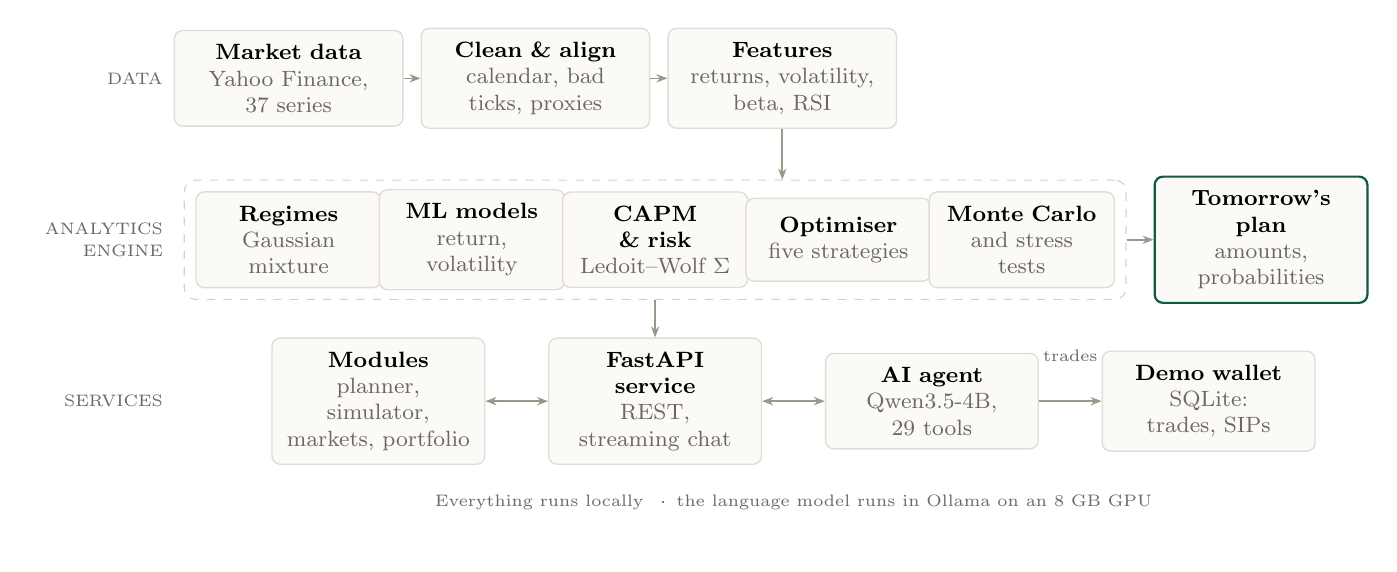
\begin{tikzpicture}[x=0.95cm, y=1cm, every node/.append style={minimum height=1.05cm}]
    % layer labels
    \node[lab, anchor=east, text width=1.6cm, align=right] at (-1.55, 0) {DATA};
    \node[lab, anchor=east, text width=1.6cm, align=right] at (-1.55, -2.05) {ANALYTICS\\ ENGINE};
    \node[lab, anchor=east, text width=1.6cm, align=right] at (-1.55, -4.1) {SERVICES};
    % row 1: data
    \node[box, text width=2.55cm] (data)  at (0, 0)    {\textbf{Market data}\\\muted{Yahoo Finance, 37 series}};
    \node[box, text width=2.55cm] (clean) at (3.3, 0)  {\textbf{Clean \& align}\\\muted{calendar, bad ticks, proxies}};
    \node[box, text width=2.55cm] (feat)  at (6.6, 0)  {\textbf{Features}\\\muted{returns, volatility, beta, RSI}};
    % row 2: engine
    \node[box, text width=2.0cm] (reg)  at (0, -2.05)    {\textbf{Regimes}\\\muted{Gaussian mixture}};
    \node[box, text width=2.0cm] (ml)   at (2.45, -2.05) {\textbf{ML models}\\\muted{return, volatility}};
    \node[box, text width=2.0cm] (capm) at (4.9, -2.05)  {\textbf{CAPM \& risk}\\\muted{Ledoit--Wolf $\Sigma$}};
    \node[box, text width=2.0cm] (opt)  at (7.35, -2.05) {\textbf{Optimiser}\\\muted{five strategies}};
    \node[box, text width=2.0cm] (mc)   at (9.8, -2.05)  {\textbf{Monte Carlo}\\\muted{and stress tests}};
    \node[fit=(reg)(mc), draw=rulec, dashed, rounded corners=4pt, inner sep=4pt, minimum height=0pt] (eng) {};
    \node[hl, text width=2.35cm] (plan) at (13.0, -2.05) {\textbf{Tomorrow's plan}\\\muted{amounts, probabilities}};
    % row 3: services
    \node[box, text width=2.35cm] (mods)   at (1.2, -4.1)  {\textbf{Modules}\\\muted{planner, simulator,\\ markets, portfolio}};
    \node[box, text width=2.35cm] (api)    at (4.9, -4.1)  {\textbf{FastAPI service}\\\muted{REST, streaming chat}};
    \node[box, text width=2.35cm] (agent)  at (8.6, -4.1)  {\textbf{AI agent}\\\muted{Qwen3.5-4B, 29 tools}};
    \node[box, text width=2.35cm] (wallet) at (12.3, -4.1) {\textbf{Demo wallet}\\\muted{SQLite: trades, SIPs}};
    % flows
    \draw[flow] (data) -- (clean);
    \draw[flow] (clean) -- (feat);
    \draw[flow] (feat.south) -- (feat.south |- eng.north);
    \draw[flow] (eng.east) -- (plan.west);
    \draw[flow] (eng.south -| api.north) -- (api.north);
    \draw[flow, {Stealth[length=4pt]}-{Stealth[length=4pt]}] (mods) -- (api);
    \draw[flow, {Stealth[length=4pt]}-{Stealth[length=4pt]}] (api) -- (agent);
    \draw[flow] (agent) -- node[lab, above=1pt]{trades} (wallet);
    \node[lab, anchor=north] at (6.75, -4.85) {Everything runs locally \enspace·\enspace the language model runs in Ollama on an 8 GB GPU};
  \end{tikzpicture}
\end{frame}

\begin{frame}{Data: Indian markets, 2014–2026}
  \vspace{0.15cm}
  \begin{columns}[T]
    \column{0.52\textwidth}
      \small
      \begin{tabularx}{\linewidth}{@{}Lr@{}}
        \toprl
        \thd{Universe} & \thd{Count}\\ \tabrule
        NSE stocks across 12 sectors (NIFTY 50 members) & 26\\
        Index ETFs: NIFTY 50, Next 50, Bank & 3\\
        Gold ETF \;·\; G-Sec bond ETF \;·\; liquid fund & 3\\ \tabrule
        Benchmark: NIFTY 50 index & 1\\
        Macro: India VIX, Brent, USD/INR, US 10Y, Bank NIFTY & 5\\ \botrl
      \end{tabularx}
      \vspace{0.35cm}

      \begin{columns}[T]
        \column{0.33\linewidth}\kpi{2,950}{trading days}
        \column{0.33\linewidth}\kpi{32}{investable assets}
        \column{0.33\linewidth}\kpi{12 yrs}{of daily OHLCV}
      \end{columns}
    \column{0.42\textwidth}
      \eyebrow{Data problems found and fixed}\par\vspace{3pt}\hair\par\vspace{5pt}
      \small
      \begin{itemize}\setlength{\itemsep}{5pt}
        \item \textbf{Wrong-scale prints} on 19--20 Dec 2019 in three ETFs (price $\div$10 to $\div$100) --- caught by a rolling-median filter.
        \item \textbf{Illiquid gilt ETF}: stale and erratic prints; tighter $\pm$4\% band around the 11-day median.
        \item \textbf{Liquid fund}: Yahoo's NAV ignores daily distributions; rebuilt from the RBI repo-rate path.
        \item All series aligned to the NSE trading calendar; small gaps forward-filled.
      \end{itemize}
  \end{columns}
\end{frame}

% ------------------------------------------------------------------ models
\section{Models}
\begin{frame}{The models at a glance}
  \vspace{0.02cm}
  \scriptsize\renewcommand{\arraystretch}{1.04}
  \begin{tabularx}{\textwidth}{@{}P{2.3cm}P{3.6cm}LP{3.05cm}@{}}
    \toprl
    \thd{Model} & \thd{Method} & \thd{Used for} & \thd{Validation}\\ \tabrule
    \textbf{Market regimes} & Gaussian mixture, 3 states: NIFTY return, vol, drawdown, VIX, 2008--26 & Today's regime; the Monte Carlo starts in it and switches by a Markov chain & After Neutral, 5\% drawdown 35\% likely vs 13\% after Calm\\ \tabrule
    \textbf{Anomaly detector} & Isolation Forest on market state; $|z| \ge 2.5$ for single stocks & Unusual market days and stock moves & Precede 21--23\% vs 13\% volatility\\ \tabrule
    \textbf{Return model} & Ridge regression, forward 21-day return & Small tilt of expected returns, weight $\lambda = 13.5\%$ from measured skill & IC 0.027; no better than the mean on error\\ \tabrule
    \textbf{Volatility model} & Ridge on realised and range-based volatility, 80/20 blend & Next-month risk of every plan and asset & $R^2$ 0.59 vs 0.50 naive\\ \tabrule
    \textbf{Expected return} & 0.6 CAPM + 0.4 clipped history + ML tilt & Drift in the optimiser and Monte Carlo & Prior, not fitted\\ \tabrule
    \textbf{Risk \& optimiser} & Ledoit--Wolf $\Sigma$, VaR, CVaR; SLSQP and LPs & Risk limits; the five strategies under caps & ---\\ \tabrule
    \textbf{Monte Carlo} & Student-$t$, regime switching, parameter uncertainty & 10,000 futures per plan & 90\% band held 81\% of 104 real outcomes\\ \botrl
  \end{tabularx}\par\vspace{0.12cm}
  {\scriptsize\muted{Random Forest, XGBoost, LightGBM and a GRU were also tested; none beat Ridge out of sample, so they are reported but not used.}}
\end{frame}

\begin{frame}{Feature engineering}
  \vspace{0.2cm}
  \begin{columns}[T]
    \column{0.47\textwidth}
      \eyebrow{Per asset, strictly backward-looking}\par\vspace{3pt}\hair\par\vspace{5pt}
      \small
      \begin{itemize}\setlength{\itemsep}{3pt}
        \item Returns over 1, 5, 21, 63, 126, 252 days
        \item Realised volatility (21, 63 days) and their ratio
        \item Range-based volatility from daily High--Low (Parkinson, Garman--Klass, Rogers--Satchell)
        \item Price vs 20/50-day averages; 50 vs 200-day
        \item RSI(14), MACD histogram, 252-day drawdown
        \item Rolling 63-day beta, correlation and skew vs NIFTY
      \end{itemize}
    \column{0.47\textwidth}
      \eyebrow{Market state (shared by all assets)}\par\vspace{3pt}\hair\par\vspace{5pt}
      \small
      \begin{itemize}\setlength{\itemsep}{3pt}
        \item NIFTY 21/63-day return, volatility, drawdown, gap to 200-day average
        \item India VIX level and 21-day change
        \item Brent, USD/INR and US 10-year moves
      \end{itemize}
      \vspace{0.25cm}
      \eyebrow{Targets}\par\vspace{3pt}\hair\par\vspace{5pt}
      Forward 21-trading-day return and next-month volatility of each asset \\[2pt]
      \muted{\footnotesize panel of 32 assets $\times$ 2,950 days}
  \end{columns}
\end{frame}

\begin{frame}{Market regimes}
  \framesubtitle{Gaussian mixture on NIFTY return, volatility, drawdown and India VIX, 2008--2026 (includes the 2008 and 2020 crashes)}
  \vspace{0.05cm}
  \centering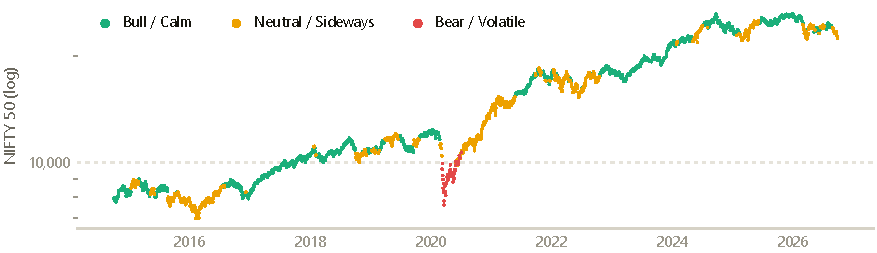
\includegraphics[width=\textwidth]{regimes.pdf}\par\vspace{0.04cm}\raggedright
  \footnotesize
  \begin{tabularx}{\textwidth}{@{}Lrrrrr@{}}
    \toprl
    \thd{Regime} & \thd{Share of days} & \thd{Return p.a.} & \thd{Volatility} & \thd{Avg VIX} & \thd{Persistence}\\ \tabrule
    \swatch{cC}\; Bull / Calm & 46\% & \up{+13.0\%} & 11.6\% & 14.1 & 96.4\%\\
    \swatch{cD}\; Neutral / Sideways \;\faint{(today)} & 45\% & \up{+5.7\%} & 18.5\% & 21.0 & 95.5\%\\
    \swatch{neg}\; Bear / Volatile & 9\% & +17.2\%$^{*}$ & 45.5\% & 42.5 & 95.4\%\\ \botrl
  \end{tabularx}
  {\scriptsize\muted{$^{*}$Crisis periods contain both the crash and the violent rebound (2009, 2020); the state is defined by 45\% volatility, VIX 42 and a $-$35\% average drawdown, not by its average return.}}
\end{frame}

\begin{frame}{Forecasting returns, honestly}
  \framesubtitle{Expanding-window walk-forward, 2021--2026, purged targets; 43,400 out-of-sample predictions}
  \vspace{0.15cm}
  \begin{columns}[T]
    \column{0.56\textwidth}
      \small
      \begin{tabularx}{\linewidth}{@{}Lrrr@{}}
        \toprl
        \thd{Model} & \thd{RMSE} & \thd{Direction} & \thd{IC}\\ \tabrule
        Ridge regression \;\textcolor{brand}{\footnotesize in use} & 0.0566 & 51.2\% & 0.027\\
        Random Forest & 0.0572 & 50.6\% & 0.001\\
        XGBoost & 0.0583 & 50.4\% & $-$0.002\\ \tabrule
        \muted{Historical mean (baseline)} & \muted{0.0565} & \muted{47.5\%} & \muted{---}\\ \botrl
      \end{tabularx}\par\vspace{0.15cm}
      {\footnotesize\muted{IC = average daily Spearman correlation between forecast and realised return across assets.}}
    \column{0.38\textwidth}
      \begin{callout}
        \textbf{No model beats the naive baseline on error.} Cross-sectional skill is at most small (IC 0.00--0.03).\par\vspace{5pt}
        So the forecast is used only as a \emph{relative tilt}, weighted by measured skill:
        \[\lambda = \mathrm{clip}(5\cdot\mathrm{IC},\,0,\,0.5) = 13.5\%\]
        A model with no skill would get zero weight automatically.
      \end{callout}
  \end{columns}
\end{frame}

\begin{frame}{Volatility is forecastable; simulated outcomes are checked against reality}
  \vspace{0.15cm}
  \begin{columns}[T]
    \column{0.5\textwidth}
      \eyebrow{Next-month volatility, walk-forward 2021--26}\par\vspace{3pt}\hair\par\vspace{2pt}
      \small
      \begin{tabularx}{\linewidth}{@{}Lrr@{}}
        \toprl
        \thd{Model} & \thd{R$^2$} & \thd{Error}\\ \tabrule
        Ridge, range-based features, 80/20 blend \;\textcolor{brand}{\footnotesize in use} & 0.59 & 25\%\\
        \muted{Same as last quarter} & \muted{0.50} & \muted{29\%}\\
        \muted{Same as last month} & \muted{0.39} & \muted{31\%}\\ \botrl
      \end{tabularx}\par\vspace{0.2cm}
      {\footnotesize\muted{40{,}423 forecasts, settings chosen on 2017--20 validation. Trees, GARCH and ensembles scored lower. Liquid fund excluded.}}
    \column{0.46\textwidth}
      \eyebrow{Monte Carlo calibration, 1-year horizon}\par\vspace{3pt}\hair\par\vspace{2pt}
      \small
      \begin{itemize}\setlength{\itemsep}{4pt}
        \item 104 forecasts from quarterly dates 2019--25, information as of each date
        \item 50 / 75 / 90 / 95 / 99\% bands held 53 / 74 / 81 / 88 / 96\% (88\% at 90\% outside 2020)
        \item The miss is the COVID crash and the rebound; realised returns beat expected by 7\% on average
        \item Adds estimation error of the expected return ($\sigma/\sqrt{5}$) and regimes learned from 2008, nothing tuned
      \end{itemize}
  \end{columns}
\end{frame}

\begin{frame}{Does the model stack create value? Walk-forward backtest, 2021--26}
  \vspace{0.1cm}
  \begin{columns}[T]
    \column{0.56\textwidth}
      \footnotesize
      \begin{tabularx}{\linewidth}{@{}Lrrrrr@{}}
        \toprl
        \thd{Strategy} & \thd{CAGR} & \thd{Vol} & \thd{Sharpe} & \thd{Max DD} & \thd{Turn./yr}\\ \tabrule
        Min-variance & 11.5\% & 5.7\% & 0.96 & $-$6.1\% & 0.8$\times$\\
        Max-Sharpe, prior & 12.8\% & 11.4\% & 0.60 & $-$16.1\% & 3.3$\times$\\
        \quad + volatility model & 14.3\% & 11.2\% & 0.74 & $-$15.2\% & 4.5$\times$\\
        \quad + 13.5\% return tilt & 14.9\% & 12.0\% & 0.75 & $-$16.9\% & 4.6$\times$\\
        \quad + regime overlay (full) & 13.8\% & 10.1\% & 0.77 & $-$13.9\% & 4.9$\times$\\ \tabrule
        \muted{NIFTY 50 ETF} & \muted{10.4\%} & \muted{12.8\%} & \muted{0.34} & \muted{$-$16.1\%} & \muted{0.2$\times$}\\
        \muted{Equal-weight stocks} & \muted{16.6\%} & \muted{13.0\%} & \muted{0.82} & \muted{$-$15.0\%} & \muted{0.7$\times$}\\ \botrl
      \end{tabularx}\par\vspace{0.12cm}
      {\footnotesize\muted{Monthly rebalance, long-only, 0.10\% cost per trade; every input uses only data available at each date.}}
    \column{0.42\textwidth}
      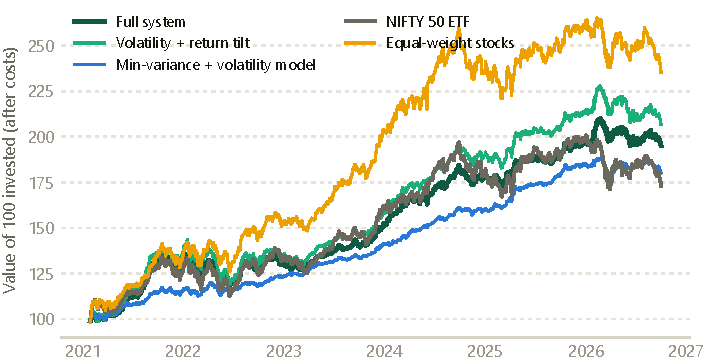
\includegraphics[width=\linewidth]{eval_curves.pdf}\par\vspace{0.08cm}
      \begin{callout}
        The volatility model and regime overlay add \emph{risk control}; the return tilt adds little. An equal-weight stock basket matches the full system in this one bull-market sample.
      \end{callout}
  \end{columns}
\end{frame}

\begin{frame}{Robustness: year by year, calibration, and what regimes and anomalies tell us}
  \vspace{0.1cm}
  \begin{columns}[T]
    \column{0.5\textwidth}
      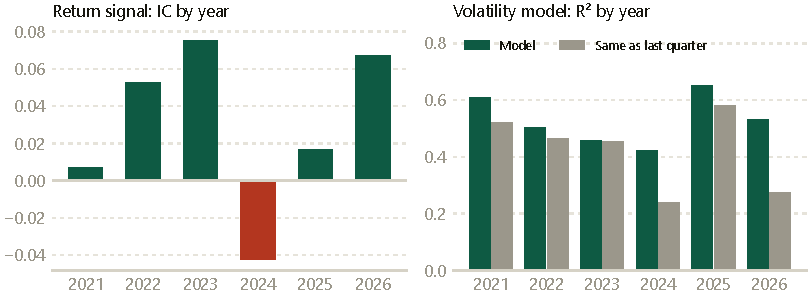
\includegraphics[width=\linewidth]{eval_by_year.pdf}\par\vspace{0.1cm}
      {\footnotesize\muted{Return signal: IC positive in 5 of 6 years, never significant on its own. Volatility model: ahead of the baseline every year (2023 narrowly).}}
    \column{0.46\textwidth}
      \small
      \begin{itemize}\setlength{\itemsep}{5pt}
        \item \textbf{Calibration.} Intervals of 50 / 75 / 90 / 95 / 99\% held 53 / 74 / 81 / 88 / 96\% (was 44 / 69 / 81 / 84 / 93). Remaining miss: the 2020 crash.
        \item \textbf{Regimes.} Calm $\to$ Neutral in a month 18\% of the time. After Neutral, 35\% of months saw a $\ge$5\% market drawdown against 13\% after Calm. VIX alone flags drawdowns as well.
        \item \textbf{Anomalies.} Flagged days are followed by 21--23\% volatility vs 13\% and a 5\% drawdown 60--65\% of the time vs 21\%, but not by lower returns: a risk warning, not a sell signal.
        \item \textbf{Return signal.} No feature set or target showed skill on 2017--20 validation; kept as a small tilt.
      \end{itemize}
  \end{columns}
\end{frame}

\begin{frame}{Expected returns and the risk model}
  \vspace{0.15cm}
  \begin{columns}[T]
    \column{0.5\textwidth}
      \eyebrow{CAPM}\par\vspace{3pt}\hair\par\vspace{2pt}
      \[ \mathbb{E}[R_i] = r_f + \beta_i\,\mathrm{ERP}, \qquad r_f = 6\% \]
      {\small ERP blends 5-year NIFTY history with a 5.5\% prior, clipped to [3\%, 8\%] $\Rightarrow$ 3.0\%, market return 9.0\%.}\par\vspace{0.25cm}
      \eyebrow{Final expected return}\par\vspace{3pt}\hair\par\vspace{2pt}
      \[ \mu_i = 0.6\,\mathrm{CAPM}_i + 0.4\,\mathrm{History}_i + \lambda\cdot\mathrm{Tilt}^{\mathrm{ML}}_i \]
    \column{0.44\textwidth}
      \eyebrow{Risk}\par\vspace{3pt}\hair\par\vspace{4pt}
      \small
      \begin{itemize}\setlength{\itemsep}{4pt}
        \item Covariance $\Sigma$: Ledoit--Wolf shrinkage on 5 years of daily returns
        \item $\mathrm{VaR}_{95}$ and $\mathrm{CVaR}_{95} = \mathbb{E}[L \mid L \ge \mathrm{VaR}]$
        \item Maximum drawdown, Sharpe $=(\mu-r_f)/\sigma$
        \item Oil and rate sensitivities for stress tests
        \item Isolation Forest flags anomalous market days
      \end{itemize}
  \end{columns}
\end{frame}

\begin{frame}{Five strategies on one efficient frontier}
  \vspace{0.05cm}
  \begin{columns}[T]
    \column{0.47\textwidth}
      \footnotesize
      \begin{tabularx}{\linewidth}{@{}p{2.85cm}L@{}}
        \toprl
        \thd{Strategy} & \thd{Optimisation}\\ \tabrule
        \swatch{cB}\; Max Return & $\max_w\, w^\top\mu$ \;(linear program)\\
        \swatch{cA}\; Min Risk & $\min_w\, w^\top\Sigma w$\\
        \swatch{cC}\; Max Sharpe & $\max_w\, (w^\top\mu - r_f)/\sqrt{w^\top\Sigma w}$\\
        \swatch{cG}\; Goal-Based & frontier point with the highest \emph{simulated} P(reach target)\\
        \swatch{cE}\; Crash-Resistant & $\min\mathrm{CVaR}_{95}$ over history \emph{and} stress scenarios (Rockafellar--Uryasev LP)\\ \botrl
      \end{tabularx}\par\vspace{0.2cm}
      {\footnotesize\muted{Long-only, fully invested; per-asset caps by risk profile (single stock 8 / 15 / 25\%); preferred sectors restrict the stock universe.}}
    \column{0.5\textwidth}
      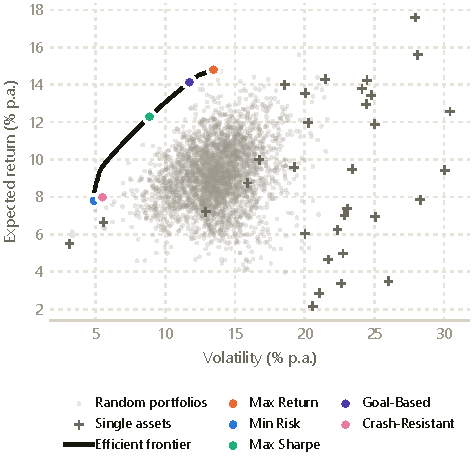
\includegraphics[width=0.86\linewidth]{frontier.pdf}
  \end{columns}
\end{frame}

\begin{frame}{Monte Carlo engine}
  \vspace{0.05cm}
  \begin{columns}[T]
    \column{0.42\textwidth}
      \small
      \begin{itemize}\setlength{\itemsep}{5pt}
        \item \textbf{10,000 daily paths} per strategy over the horizon
        \item \textbf{Fat tails}: Student-$t$ innovations, $\nu = 5$
        \item \textbf{Regime switching}: 3-state Markov chain from the GMM transition matrix, started from today's regime
        \item \textbf{Parameter uncertainty}: each path draws its own expected return ($\pm\sigma/\sqrt{5}$)
        \item \textbf{Day-0 shocks} move the market into the bear regime
        \item Outputs: P(gain), P(target), VaR, CVaR, drawdowns, percentile bands
      \end{itemize}
    \column{0.55\textwidth}
      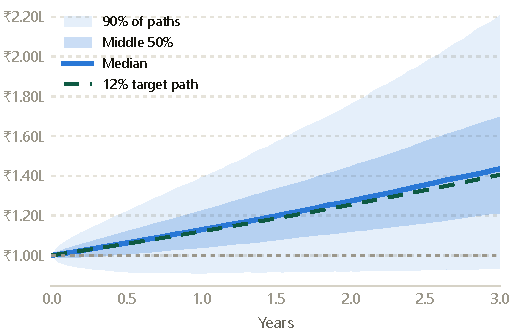
\includegraphics[width=\linewidth]{fan.pdf}\par
      {\footnotesize\muted{Recommended plan, ₹1,00,000 over 3 years: median, middle 50\% and 90\% of paths against the 12\% target path.}}
  \end{columns}
\end{frame}

% ------------------------------------------------------------------ results
\section{Results}
\begin{frame}{Tomorrow's investment plan}
  \framesubtitle{Sample investor: ₹1,00,000 \;·\; 3 years \;·\; medium risk \;·\; 12\% target \;·\; prices at the close of 1 Oct 2026}
  \vspace{0.1cm}
  \begin{columns}[T]
    \column{0.47\textwidth}
      {\displayfont\fontsize{19}{22}\selectfont Goal-Based \; {\fontsize{7}{8}\selectfont\sffamily\color{brand}\addfontfeature{LetterSpace=10}RECOMMENDED}\par}\vspace{3pt}
      {\footnotesize\muted{Within medium-risk limits; its 53\% chance of reaching 12\% ties Max Return (within 2 pp) and it has the higher Sharpe ratio.}}\par\vspace{0.2cm}
      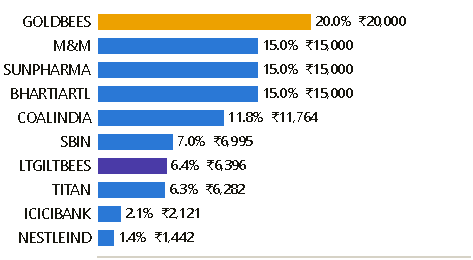
\includegraphics[width=0.96\linewidth]{allocation.pdf}\par
      {\footnotesize\swatch{cA}\,Stocks 76\% \quad \swatch{cD}\,Gold 20\% \quad \swatch{faint}\,Cash \faint{\& residual}}
    \column{0.47\textwidth}
      \vspace{0.35cm}
      \begin{columns}[T]
        \column{0.5\linewidth}\kpi{14.1\%}{Expected return}\par\vspace{9pt}\kpi{91\%}{Chance of gain}\par\vspace{9pt}\kpi{15.0\%}{Expected drawdown}
        \column{0.5\linewidth}\kpi{12.3\%}{Volatility}\par\vspace{9pt}\kpi{53\%}{Reach 12\% target}\par\vspace{9pt}\kpi{8 of 9}{Stress tests passed}
      \end{columns}
      \vspace{0.3cm}\hair\par\vspace{3pt}
      {\footnotesize Sharpe 0.66 \;·\; beta 0.69 \;·\; 1-year VaR\textsubscript{95} 9.4\% \;·\; CVaR\textsubscript{95} 15.1\%\par
       \muted{Whole shares at the latest close, after 0.1\% trading costs.}}
  \end{columns}
\end{frame}

\begin{frame}{What could happen: the distribution, not a point}
  \vspace{0.05cm}
  \begin{columns}[T]
    \column{0.55\textwidth}
      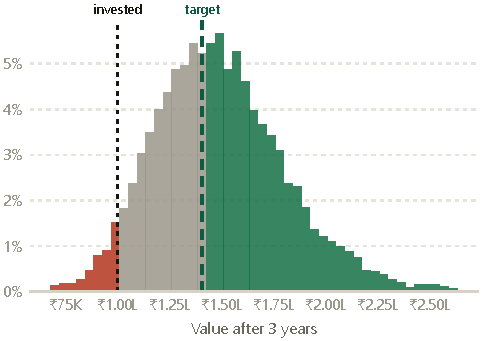
\includegraphics[width=\linewidth]{distribution.pdf}\par
      {\footnotesize\swatch{pos}\;target met \quad\swatch{faint}\;gain, below target \quad\swatch{neg}\;loss}
    \column{0.4\textwidth}
      \vspace{0.2cm}
      \eyebrow{Value after 3 years}\par\vspace{3pt}\hair\par\vspace{4pt}
      \begin{tabularx}{\linewidth}{@{}Lr@{}}
        Worst 5\% & {\numfont ₹91,984}\\
        \textbf{Median} & {\numfont\textbf{₹1,42,950}}\\
        Best 5\% & {\numfont ₹2,24,745}\\
      \end{tabularx}\par\vspace{0.3cm}
      \eyebrow{Proposal's illustration vs system output}\par\vspace{3pt}\hair\par\vspace{2pt}
      \footnotesize
      \begin{tabularx}{\linewidth}{@{}Lrr@{}}
        & \thd{Proposal} & \thd{System}\\
        Expected return & $\sim$12.4\% & 14.1\%\\
        Volatility & $\sim$14.2\% & 12.3\%\\
        P(positive) & $\sim$73\% & 91\%\\
        P(target) & $\sim$68\% & 53\%\\
      \end{tabularx}
  \end{columns}
\end{frame}

\begin{frame}{Five strategies compared}
  \framesubtitle{Same investor, same 10,000 simulated futures for every strategy}
  \vspace{0.25cm}
  \small
  \begin{tabularx}{\textwidth}{@{}Lrrrrrr@{}}
    \toprl
    \thd{Strategy} & \thd{Return} & \thd{Volatility} & \thd{Sharpe} & \thd{Chance of gain} & \thd{Reach target} & \thd{Median value}\\ \tabrule
    \swatch{cB}\; Max Return & 14.8\% & 14.2\% & 0.62 & 88\% & \textbf{53\%} & ₹1,43,902\\
    \swatch{cA}\; Min Risk & 7.1\% & 4.9\% & 0.22 & 97\% & 10\% & ₹1,21,981\\
    \swatch{cC}\; Max Sharpe & 12.4\% & 9.6\% & \textbf{0.67} & 94\% & 48\% & ₹1,38,878\\
    \swatch{cG}\; \textbf{Goal-Based} \;\textcolor{brand}{\footnotesize recommended} & 14.1\% & 12.3\% & 0.66 & 91\% & \textbf{53\%} & ₹1,42,950\\
    \swatch{cE}\; Crash-Resistant & 7.4\% & 5.5\% & 0.25 & 96\% & 13\% & ₹1,22,890\\ \botrl
  \end{tabularx}
  \vspace{0.45cm}
  \begin{callout}
    \textbf{Decision rule.} Keep strategies inside the investor's limits on volatility, worst stress loss and one-year VaR;
    pick the highest probability of reaching the target; within 2 percentage points prefer the higher Sharpe ratio.
    Defensive strategies are almost certain to gain but rarely reach a 12\% goal.
  \end{callout}
\end{frame}

\begin{frame}{Stress tests}
  \vspace{0.05cm}
  \begin{columns}[T]
    \column{0.58\textwidth}
      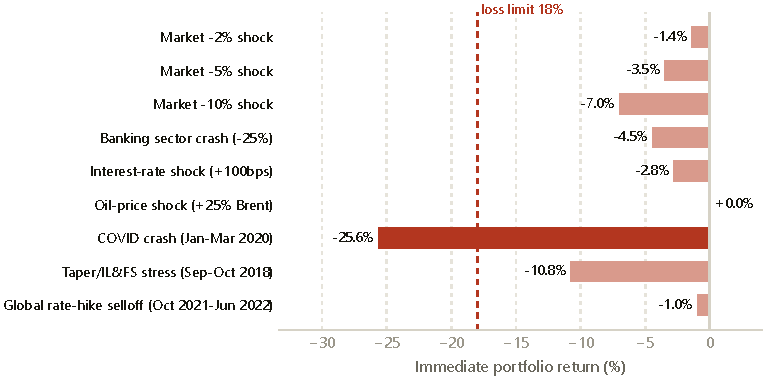
\includegraphics[width=\linewidth]{stress.pdf}
    \column{0.37\textwidth}
      \eyebrow{Monte Carlo after a day-0 shock}\par\vspace{3pt}\hair\par\vspace{3pt}
      \footnotesize
      \begin{tabularx}{\linewidth}{@{}Lrr@{}}
        \thd{Scenario} & \thd{Median} & \thd{P(tgt)}\\
        No shock & ₹1,43,658 & 53\%\\
        Market $-$2\% & ₹1,41,662 & 51\%\\
        Market $-$5\% & ₹1,39,018 & 48\%\\
        Market $-$10\% & ₹1,34,016 & 43\%\\
        Pharma crash & ₹1,37,741 & 47\%\\
        Rate +100 bp & ₹1,40,368 & 50\%\\
        Oil +25\% & ₹1,43,940 & 53\%\\
      \end{tabularx}\par\vspace{0.2cm}
      {\footnotesize\muted{Only a COVID-scale crash (\dn{$-$24.8\%}) breaches the 18\% medium-risk loss limit.}}
  \end{columns}
\end{frame}

\begin{frame}{Invest now, wait, or SIP?}
  \framesubtitle{All options run on the same simulated markets; uninvested money earns the risk-free rate}
  \vspace{0.25cm}
  \begin{columns}[T]
    \column{0.56\textwidth}
      \small
      \begin{tabularx}{\linewidth}{@{}Lrr@{}}
        \toprl
        \thd{Option} & \thd{Median after 3 yr} & \thd{Beats lump sum}\\ \tabrule
        \textbf{Invest now (lump sum)} & \textbf{₹1,42,159} & ---\\
        Wait 1 month & ₹1,41,682 & 45\%\\
        Wait 3 months & ₹1,40,628 & 39\%\\
        Wait 6 months & ₹1,38,473 & 36\%\\
        SIP over 6 months & ₹1,40,958 & 39\%\\
        SIP over 12 months & ₹1,39,134 & 35\%\\ \botrl
      \end{tabularx}
    \column{0.38\textwidth}
      \vspace{0.2cm}
      \begin{callout}
        With a positive expected return, \textbf{time in the market beats timing it}: every delay lowers the median outcome.\par\vspace{5pt}
        A SIP is still useful when the investor values a narrower range of bad outcomes over the higher median --- it wins in about a third of futures.
      \end{callout}
  \end{columns}
\end{frame}

\begin{frame}{Walk-forward backtest}
  \framesubtitle{Weights chosen only from data before 3 Oct 2023, rebalanced quarterly, held to 1 Oct 2026; no ML (no look-ahead)}
  \vspace{0.05cm}
  \centering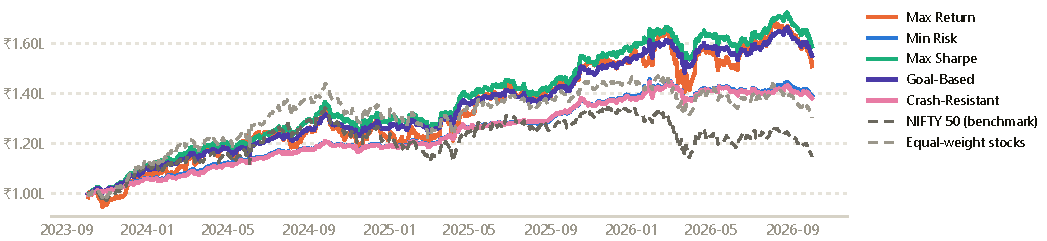
\includegraphics[width=\textwidth]{backtest.pdf}\par\vspace{0.05cm}\raggedright
  \footnotesize
  \begin{tabularx}{\textwidth}{@{}Lrrrrr@{}}
    \toprl
    \thd{Strategy} & \thd{Total return} & \thd{CAGR} & \thd{Volatility} & \thd{Sharpe} & \thd{Max drawdown}\\ \tabrule
    \swatch{cG}\; Goal-Based & \up{+55.1\%} & 16.1\% & 8.9\% & \textbf{1.14} & $-$8.1\%\\
    \swatch{cC}\; Max Sharpe & \up{+58.8\%} & 17.1\% & 10.3\% & 1.07 & $-$9.3\%\\
    \swatch{cA}\; Min Risk \;/\; \swatch{cE}\; Crash-Resistant & \up{+39.1\%} \;/\; \up{+38.1\%} & 11.9 / 11.6\% & 5.9 / 6.0\% & 1.00 / 0.95 & $-$6.8 / $-$6.3\%\\
    \muted{NIFTY 50 benchmark} & \muted{+14.8\%} & \muted{4.8\%} & \muted{13.3\%} & \muted{$-$0.09} & \muted{$-$15.8\%}\\ \botrl
  \end{tabularx}
\end{frame}

% ------------------------------------------------------------------ modules
\section{Modules}
\begin{frame}{Planner: tomorrow's plan for a profile}
  \vspace{0.2cm}
  \begin{columns}[T]
    \column{0.3\textwidth}
      \eyebrow{Inputs}\par\vspace{3pt}\hair\par\vspace{4pt}
      \footnotesize
      \begin{itemize}\setlength{\itemsep}{3pt}
        \item Amount in rupees
        \item Horizon: 1, 3 or 5 years
        \item Risk tolerance: low, medium, high
        \item Target return: 4--30\% a year
        \item Preferred sectors (optional): restrict which stocks may be used; Gold / Bonds force at least 10\%
      \end{itemize}
    \column{0.33\textwidth}
      \eyebrow{What it computes}\par\vspace{3pt}\hair\par\vspace{4pt}
      \footnotesize
      \begin{enumerate}\setlength{\itemsep}{3pt}
        \item The five strategies under the profile's caps
        \item 10,000 futures and 9 stress scenarios for each
        \item Risk-limit check: volatility, worst stress loss, 1-year VaR
        \item Recommendation by the decision rule
        \item Whole-share plan at the latest close, costs reserved
      \end{enumerate}
    \column{0.3\textwidth}
      \eyebrow{Outputs, per strategy}\par\vspace{3pt}\hair\par\vspace{4pt}
      \footnotesize
      \begin{itemize}\setlength{\itemsep}{3pt}
        \item Allocation: weight, rupees, shares, cash left
        \item Expected return, volatility, chance of gain, chance of target, drawdown
        \item Monte Carlo bands, stress results, now vs wait vs SIP, backtest
        \item \textbf{Invest this plan} --- one order set for the demo wallet
      \end{itemize}
  \end{columns}
  \vspace{0.35cm}
  {\footnotesize\renewcommand{\arraystretch}{1.1}
  \begin{tabularx}{\textwidth}{@{}Lrrrrr@{}}
    \toprl
    \thd{Risk profile} & \thd{Single stock cap} & \thd{Index ETF cap} & \thd{Max volatility} & \thd{Max stress loss} & \thd{Max 1-yr VaR}\\ \tabrule
    Low \;/\; Medium \;/\; High & 8 / 15 / 25\% & 30 / 35 / 40\% & 11 / 15 / 22\% & 10 / 18 / 30\% & 8 / 15 / 28\%\\ \botrl
  \end{tabularx}}
\end{frame}

\begin{frame}{Simulator: “what could my own mix become?”}
  \vspace{0.2cm}
  \begin{columns}[T]
    \column{0.47\textwidth}
      \eyebrow{The question it answers}\par\vspace{3pt}\hair\par\vspace{4pt}
      \small
      “If I put ₹X now, and optionally ₹Y every month, into \emph{these} assets, what could it be worth each year for the next 1--10 years?”\par\vspace{0.3cm}
      \eyebrow{How}\par\vspace{3pt}\hair\par\vspace{4pt}
      \footnotesize
      \begin{itemize}\setlength{\itemsep}{3pt}
        \item Any mix of the 32 assets with any weights (scaled to 100\%), or a starting point: recommended plan, NIFTY 50, balanced, gold, IT leaders, banking, capital preservation
        \item The same fat-tailed, regime-switching Monte Carlo as the planner
        \item Monthly contributions are added at each month end and grow from their own date
      \end{itemize}
    \column{0.47\textwidth}
      \eyebrow{What it reports}\par\vspace{3pt}\hair\par\vspace{4pt}
      \footnotesize
      \begin{itemize}\setlength{\itemsep}{3pt}
        \item Year by year: money put in, worst 5\%, median, best 5\%, chance of profit
        \item Expected and median final value; median annual return (money-weighted when there is a SIP)
        \item Chance of beating a fixed deposit at 6\% and the NIFTY at its expected 9\%
        \item Chance of losing 10\% or more
        \item Per-asset breakdown: share, expected return, volatility, contribution
      \end{itemize}
      \vspace{0.15cm}
      \begin{callout}
        Example: ₹1 lakh plus ₹10,000 a month for 10 years in 60\% NIFTY, 25\% gold, 15\% gilts --- ₹13 lakh put in, median ₹19.0 lakh, 90\% chance of profit, 57\% chance of beating a fixed deposit.
      \end{callout}
  \end{columns}
\end{frame}

\begin{frame}{Markets: the market, read by the models}
  \vspace{0.2cm}
  \begin{columns}[T]
    \column{0.31\textwidth}
      \eyebrow{Market snapshot}\par\vspace{3pt}\hair\par\vspace{4pt}
      \footnotesize NIFTY level and 1-day, 1-month, 1-year change; distance from the high; India VIX and 1-month volatility; today's regime with its probability; anomaly flag and unusual stock moves ($|z| \ge 2.5$).\par\vspace{0.3cm}
      \eyebrow{Regimes \& anomalies}\par\vspace{3pt}\hair\par\vspace{4pt}
      \footnotesize NIFTY since 2014 coloured by regime; anomaly score of every day, with flagged days.
    \column{0.31\textwidth}
      \eyebrow{Asset analytics (each of 32)}\par\vspace{3pt}\hair\par\vspace{4pt}
      \footnotesize
      \begin{itemize}\setlength{\itemsep}{2pt}
        \item Price, 1-month and 1-year return
        \item Beta, CAPM and model expected return
        \item Volatility and next-month forecast
        \item Daily VaR\textsubscript{95} and CVaR\textsubscript{95}, 5-year max drawdown and Sharpe
        \item RSI(14), above or below the 200-day average
        \item ML forecast for the next 21 days
      \end{itemize}
    \column{0.31\textwidth}
      \eyebrow{Correlation}\par\vspace{3pt}\hair\par\vspace{4pt}
      \footnotesize Heat map of all asset correlations --- shows why gold and gilts diversify an equity-heavy plan.\par\vspace{0.3cm}
      \eyebrow{Model validation}\par\vspace{3pt}\hair\par\vspace{4pt}
      \footnotesize Walk-forward scores of every return and volatility model against its baselines, and regime statistics --- the evidence behind each number the engine uses.
  \end{columns}
\end{frame}

\begin{frame}{Portfolio: the demo wallet}
  \vspace{0.2cm}
  \begin{columns}[T]
    \column{0.47\textwidth}
      \eyebrow{Account}\par\vspace{3pt}\hair\par\vspace{4pt}
      \footnotesize
      ₹10,00,000 of virtual cash in a local SQLite database. Orders fill at the latest close with 0.05\% brokerage + 0.05\% slippage;
      a set of orders executes all-or-nothing, and a sell can never exceed the holding nor a buy the cash.\par\vspace{0.3cm}
      \eyebrow{What it tracks}\par\vspace{3pt}\hair\par\vspace{4pt}
      \begin{itemize}\setlength{\itemsep}{2pt}
        \item Portfolio value, cash, invested value, unrealised P\&L
        \item Every holding: quantity, average cost, price, value, P\&L
        \item Value over time and the full trade history
      \end{itemize}
    \column{0.47\textwidth}
      \eyebrow{What it can do}\par\vspace{3pt}\hair\par\vspace{4pt}
      \footnotesize
      \begin{tabularx}{\linewidth}{@{}p{2.3cm}L@{}}
        \textbf{Invest the plan} & buy every asset of tomorrow's plan\\ \tabrule
        \textbf{Trade} & buy or sell one asset by quantity or rupees; sell everything\\ \tabrule
        \textbf{Rebalance} & back to a strategy's target weights\\ \tabrule
        \textbf{Health check} & review only, proposes orders\\ \tabrule
        \textbf{Auto-manage} & executes what the health check proposes\\ \tabrule
        \textbf{SIPs} & monthly instalments into a strategy; next one runs when a new month of data arrives\\ \tabrule
        \textbf{Funds} & add virtual money; reset to ₹10 lakh\\
      \end{tabularx}
  \end{columns}
\end{frame}

% ------------------------------------------------------------------ agent
\section{AI agent}
\begin{frame}{What the agent does}
  \framesubtitle{One conversation covers the whole system: 29 tools, each a real engine or wallet function}
  \vspace{0.12cm}
  \scriptsize\renewcommand{\arraystretch}{1.1}
  \begin{tabularx}{\textwidth}{@{}P{4.3cm}LP{3.7cm}@{}}
    \toprl
    \thd{Investor says} & \thd{What the agent does} & \thd{Tools}\\ \tabrule
    “₹2 lakh, 3 years, medium risk, 12\%, I like IT and banking” & saves the profile, builds and explains tomorrow's plan & \tool{set\_profile}, \tool{get\_investment\_plan}\\ \tabrule
    “Compare the strategies” \;·\; “What's my chance of the target?” & five-strategy table; Monte Carlo probabilities and best / median / worst & \tool{compare\_strategies}, \tool{run\_monte\_carlo}\\ \tabrule
    “Stress test it” \;·\; “Now, wait or SIP?” \;·\; “Backtest it” & shocks and crash replays; timing comparison; walk-forward backtest & \tool{stress\_test}, \tool{compare\_timing}, \tool{run\_backtest}\\ \tabrule
    “How is the market?” \;·\; “Tell me about TCS” & regime, VIX, anomalies; full risk and return analysis of one asset & \tool{get\_market\_overview}, \tool{analyze\_asset}\\ \tabrule
    “Invest it” \;·\; “Sell all my TCS” \;·\; “Rebalance” & places the orders in the demo wallet (next slides) & \tool{invest\_plan}, \tool{trade}, \tool{rebalance\_portfolio}\\ \tabrule
    “Check my portfolio” \;·\; “Manage it” & health check; then stop-loss, trim, de-risk, deploy cash & \tool{check\_portfolio}, \tool{auto\_manage\_portfolio}\\ \tabrule
    “Start a SIP of ₹10,000 for 12 months” & first instalment now, the rest monthly; projections and stop & \tool{start\_sip}, \tool{project\_sip}, \tool{stop\_sip}\\ \tabrule
    “Switch to ask-first” \;·\; “confirm” & changes autonomy; executes staged orders only on confirmation & \tool{set\_autonomy}, \tool{confirm\_pending\_order}\\ \botrl
  \end{tabularx}
\end{frame}

\begin{frame}{How the agent works}
  \framesubtitle{Qwen3.5-4B, local through Ollama: the model picks tools and explains; the engine produces every number}
  \vspace{0.0cm}
  \centering
  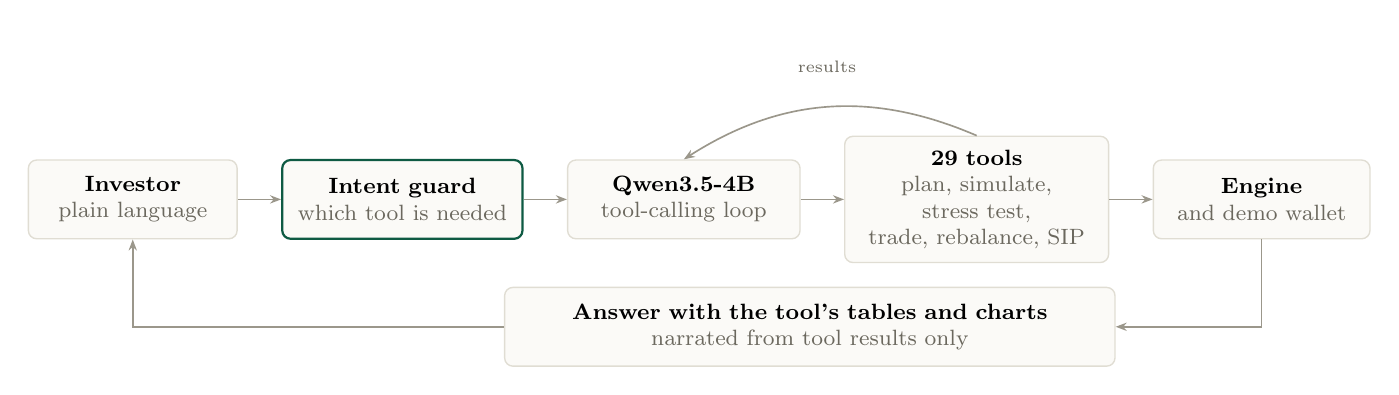
\begin{tikzpicture}[node distance=0.5cm]
    \tikzset{every node/.append style={minimum height=1.0cm}}
    \node[box, text width=2.3cm] (u) {\textbf{Investor}\\\muted{plain language}};
    \node[hl, text width=2.7cm, right=0.55cm of u] (g) {\textbf{Intent guard}\\\muted{which tool is needed}};
    \node[box, text width=2.6cm, right=0.55cm of g] (l) {\textbf{Qwen3.5-4B}\\\muted{tool-calling loop}};
    \node[box, text width=3.0cm, right=0.55cm of l] (t) {\textbf{29 tools}\\\muted{plan, simulate, stress test,\\ trade, rebalance, SIP}};
    \node[box, text width=2.4cm, right=0.55cm of t] (e) {\textbf{Engine}\\\muted{and demo wallet}};
    \node[box, text width=7.4cm, below=0.6cm of l, xshift=1.6cm] (o) {\textbf{Answer with the tool's tables and charts}\\\muted{narrated from tool results only}};
    \draw[flow] (u)--(g); \draw[flow] (g)--(l); \draw[flow] (l)--(t); \draw[flow] (t)--(e);
    \draw[flow] (e.south) |- (o.east);
    \draw[flow] (t.north) to[bend right=28] node[lab, above]{results} (l.north);
    \draw[flow] (o.west) -| (u.south);
  \end{tikzpicture}
  \vspace{0.1cm}
  \begin{columns}[T]
    \column{0.31\textwidth}
      \eyebrow{Grounding}\par\vspace{3pt}\hair\par\vspace{3pt}
      {\footnotesize If a request needs a tool and the model skips it, the agent runs the tool itself; the model only narrates the result.}
    \column{0.31\textwidth}
      \eyebrow{Words come from the user}\par\vspace{3pt}\hair\par\vspace{3pt}
      {\footnotesize Amounts, durations, strategy names and the mode are read from the investor's message, never invented by the model.}
    \column{0.31\textwidth}
      \eyebrow{Measured}\par\vspace{3pt}\hair\par\vspace{3pt}
      {\footnotesize \textbf{23 / 23} scripted conversations pass with the live model: analysis, trading, stop-loss, ask-first.}
  \end{columns}
\end{frame}

\begin{frame}{What happens in auto-trade}
  \framesubtitle{Example: auto-trade on, the investor writes “invest it”}
  \vspace{0.15cm}
  \begin{columns}[T]
    \column{0.185\textwidth}
      \stepn{1}\par\vspace{2pt}\hair\par\vspace{4pt}
      {\small\textbf{Read intent}\par}\vspace{2pt}
      {\scriptsize\muted{Code classifies the message: an \emph{instruction} (“invest it”) or a \emph{question} (“should I?”). Questions never trade.}}
    \column{0.185\textwidth}
      \stepn{2}\par\vspace{2pt}\hair\par\vspace{4pt}
      {\small\textbf{Pick the tool}\par}\vspace{2pt}
      {\scriptsize\muted{“Invest” $\Rightarrow$ invest\_plan, “sell” $\Rightarrow$ trade, “rebalance”, “manage” $\Rightarrow$ theirs; forced if the model hesitates.}}
    \column{0.185\textwidth}
      \stepn{3}\par\vspace{2pt}\hair\par\vspace{4pt}
      {\small\textbf{Size the orders}\par}\vspace{2pt}
      {\scriptsize\muted{Current plan in whole shares at the latest close; amount from the user's words, capped at cash.}}
    \column{0.185\textwidth}
      \stepn{4}\par\vspace{2pt}\hair\par\vspace{4pt}
      {\small\textbf{Execute}\par}\vspace{2pt}
      {\scriptsize\muted{Auto mode + instruction $\Rightarrow$ all orders fill together; any failure rolls back the whole set.}}
    \column{0.185\textwidth}
      \stepn{5}\par\vspace{2pt}\hair\par\vspace{4pt}
      {\small\textbf{Report}\par}\vspace{2pt}
      {\scriptsize\muted{Orders, cash left and wallet value; the agent may only claim what the tool executed.}}
  \end{columns}
  \vspace{0.55cm}
  \begin{columns}[T]
    \column{0.47\textwidth}
      \eyebrow{Still staged, even in auto-trade}\par\vspace{3pt}\hair\par\vspace{4pt}
      \footnotesize
      \begin{itemize}\setlength{\itemsep}{2pt}
        \item a question (“should I invest now?”) --- analysis only
        \item the word “stage” in the message
        \item a wallet reset, which always needs “reset” and a confirmation
      \end{itemize}
    \column{0.47\textwidth}
      \begin{callout}
        Every guard is checked in code, not by the language model: a misbehaving model can at worst \emph{fail} to trade, never trade without an instruction.
      \end{callout}
  \end{columns}
\end{frame}

\begin{frame}{Ask-first mode, autopilot and auto-manage}
  \vspace{0.15cm}
  \begin{columns}[T]
    \column{0.47\textwidth}
      \eyebrow{Ask-first mode}\par\vspace{3pt}\hair\par\vspace{4pt}
      \small
      Every order is \textbf{staged}, never executed. The agent lists the staged orders; they execute only when the investor's own next message confirms (“yes, confirm”), checked in code. “Cancel” discards them.\par\vspace{0.3cm}
      \eyebrow{Autopilot}\par\vspace{3pt}\hair\par\vspace{4pt}
      Runs the health check and auto-manage as soon as it is switched on and after every market-data refresh --- the portfolio is managed without a message. Due SIP instalments are invested at the same time.
    \column{0.47\textwidth}
      \eyebrow{Health check \& auto-manage rules}\par\vspace{3pt}\hair\par\vspace{2pt}
      \footnotesize
      \begin{tabularx}{\linewidth}{@{}p{2.1cm}L@{}}
        \textbf{Stop-loss} & position down 15\% from cost $\Rightarrow$ sell it\\ \tabrule
        \textbf{Drift} & holding 3 pp above its cap, or outside the preferred sectors $\Rightarrow$ trim\\ \tabrule
        \textbf{Risk limit} & volatility $>$ 1.1$\times$ limit $\Rightarrow$ rebalance to the plan (to Min Risk if $>$ 1.5$\times$)\\ \tabrule
        \textbf{Bear regime} & equity $>$ 60\% (low/medium risk) $\Rightarrow$ move to Crash-Resistant\\ \tabrule
        \textbf{Idle cash} & $>$ 25\% of the wallet $\Rightarrow$ deploy into the recommended plan\\
      \end{tabularx}\par\vspace{0.2cm}
      {\footnotesize\muted{The health check only proposes; auto-manage executes, under the same autonomy rules.}}
  \end{columns}
\end{frame}

\section{Verification}
\begin{frame}{Engineering and verification}
  \vspace{0.15cm}
  \begin{columns}[T]
    \column{0.31\textwidth}
      \eyebrow{Stack}\par\vspace{3pt}\hair\par\vspace{4pt}
      \footnotesize
      Python 3.13 \;·\; pandas, scikit-learn, XGBoost, PyTorch, SciPy\par\vspace{3pt}
      FastAPI service with streaming chat\par\vspace{3pt}
      Ollama + Qwen3.5-4B (RTX 4070, 8 GB)\par\vspace{3pt}
      SQLite demo wallet\par\vspace{3pt}
      Docker Compose deployment
    \column{0.31\textwidth}
      \kpi{81}{unit tests passing}\par\vspace{9pt}
      \kpi{29}{API endpoint checks}\par\vspace{9pt}
      \kpi{23 / 23}{agent conversation cases}
    \column{0.31\textwidth}
      \eyebrow{What the tests cover}\par\vspace{3pt}\hair\par\vspace{4pt}
      \footnotesize
      CAPM, VaR/CVaR and drawdown maths; optimiser constraints for every risk level; Monte Carlo mean and shock behaviour; wallet accounting;
      trade intent detection; confirmation, stop-loss and SIP guards; strategy and mode selection from the user's words.\par\vspace{0.35cm}
      \muted{Code: github.com/Tendool/If-I-invest-tomorrow}
  \end{columns}
\end{frame}

% ------------------------------------------------------------------ close
\section{Close}
\begin{frame}{Limitations}
  \vspace{0.2cm}
  \begin{columns}[T]
    \column{0.47\textwidth}
      \small
      \begin{itemize}\setlength{\itemsep}{6pt}
        \item \textbf{Weak predictability}: monthly returns are close to unforecastable; the ML adds only a small tilt.
        \item \textbf{Assumptions}: risk-free rate 6\%, ERP prior, sector rate sensitivities and bond duration are set by hand.
        \item \textbf{One backtest window}: NIFTY was weak over 2023--26 in this data, which flatters diversified portfolios.
      \end{itemize}
    \column{0.47\textwidth}
      \small
      \begin{itemize}\setlength{\itemsep}{6pt}
        \item \textbf{Data}: Yahoo Finance prices; the liquid fund is a reconstructed proxy; no taxes (STT, capital gains).
        \item \textbf{Small language model}: occasional slips in wording; the tool tables attached to each answer are authoritative.
        \item \textbf{Simulation only}: demo money, not investment advice.
      \end{itemize}
  \end{columns}
\end{frame}

\begin{frame}{Future work}
  \vspace{0.2cm}
  \begin{columns}[T]
    \column{0.31\textwidth}
      \eyebrow{Signals}\par\vspace{3pt}\hair\par\vspace{4pt}
      \small News sentiment with FinBERT as a model feature; macro factors from RBI data; Black--Litterman views instead of a fixed blend.
    \column{0.31\textwidth}
      \eyebrow{Realism}\par\vspace{3pt}\hair\par\vspace{4pt}
      \small Indian tax and transaction costs; mutual funds as SIP products; multi-period rebalancing; intraday data.
    \column{0.31\textwidth}
      \eyebrow{Agent}\par\vspace{3pt}\hair\par\vspace{4pt}
      \small Benchmark 7--9B local models on the same 23 cases; scheduled autopilot; explanation of each trade in the history.
  \end{columns}
\end{frame}

\begin{frame}{Conclusion}
  \vspace{0.3cm}
  {\displayfont\fontsize{19}{25}\selectfont From \emph{“what might happen”} to \emph{“what to do tomorrow”}.\par}
  \vspace{0.45cm}
  \begin{columns}[T]
    \column{0.31\textwidth}
      \kpi[brand]{1}{integrated pipeline}\par\vspace{4pt}
      {\footnotesize Data, ML, CAPM, optimisation, Monte Carlo and stress testing in one system.}
    \column{0.31\textwidth}
      \kpi[brand]{5}{strategies, one rule}\par\vspace{4pt}
      {\footnotesize Compared on the same futures and chosen transparently against the investor's limits.}
    \column{0.31\textwidth}
      \kpi[brand]{1}{agent that acts}\par\vspace{4pt}
      {\footnotesize Plans, simulates, invests, sells, rebalances and runs SIPs --- grounded in the engine, guarded in code.}
  \end{columns}
  \vspace{0.5cm}
  \begin{callout}
    The honest finding matters as much as the plan: forecasting single-month returns barely beats a naive baseline, so the
    value of the system lies in measuring risk, comparing strategies and showing the full range of outcomes.
  \end{callout}
\end{frame}

\begin{frame}{References}
  \vspace{0.1cm}
  \footnotesize
  \begin{enumerate}\setlength{\itemsep}{2.5pt}
    \item Markowitz, H. --- Portfolio Selection. \emph{Journal of Finance}, 1952.
    \item Sharpe, W. F. --- Capital Asset Prices: A Theory of Market Equilibrium under Conditions of Risk. \emph{Journal of Finance}, 1964.
    \item Glasserman, P. --- \emph{Monte Carlo Methods in Financial Engineering}. Springer, 2004.
    \item Hull, J. C. --- \emph{Options, Futures, and Other Derivatives}. Pearson.
    \item Hochreiter, S. \& Schmidhuber, J. --- Long Short-Term Memory. \emph{Neural Computation}, 1997.
    \item Ledoit, O. \& Wolf, M. --- A Well-Conditioned Estimator for Large-Dimensional Covariance Matrices. \emph{Journal of Multivariate Analysis}, 2004.
    \item Rockafellar, R. T. \& Uryasev, S. --- Optimization of Conditional Value-at-Risk. \emph{Journal of Risk}, 2000.
    \item Hamilton, J. D. --- A New Approach to the Economic Analysis of Nonstationary Time Series and the Business Cycle. \emph{Econometrica}, 1989.
    \item Liu, F. T., Ting, K. M. \& Zhou, Z.-H. --- Isolation Forest. \emph{IEEE ICDM}, 2008.
    \item Chen, T. \& Guestrin, C. --- XGBoost: A Scalable Tree Boosting System. \emph{KDD}, 2016.
    \item Cho, K. et al. --- Learning Phrase Representations using RNN Encoder--Decoder (GRU). \emph{EMNLP}, 2014.
  \end{enumerate}
\end{frame}

\begin{frame}[plain]
  \vspace*{2.2cm}
  \hspace*{0.15cm}\begin{minipage}{0.9\textwidth}
    {\displayfont\fontsize{38}{40}\selectfont Thank \textit{you}\par}\vspace{0.3cm}
    {\fontsize{13}{16}\selectfont\color{muted}Questions and live demo\par}\vspace{0.7cm}
    {\color{rulec}\rule{\linewidth}{0.4pt}}\par\vspace{0.25cm}
    {\small\color{muted}Rupali K \enspace·\enspace Mahadev S \enspace·\enspace Srivatsav S \enspace·\enspace Sarang U \hfill github.com/Tendool/If-I-invest-tomorrow}
  \end{minipage}
\end{frame}

\end{document}
